% Author: Grayson Orr
% Course: IN721: Mobile Application Development

\documentclass{article}
\author{}

\usepackage{graphicx}
\usepackage{wrapfig}
\usepackage{enumerate}
\usepackage{hyperref}
\usepackage[margin = 2.25cm]{geometry}
\usepackage[table]{xcolor}
\usepackage{fancyhdr}
\hypersetup{
  colorlinks = true,
  urlcolor = blue
}
\setlength\parindent{0pt}
\pagestyle{fancy}
\fancyhf{}
\rhead{College of Engineering, Construction and Living Sciences\\Bachelor of Information Technology}
\lfoot{Practical 02: Calculator\\Version 1, Semester One, 2020}
\rfoot{\thepage}

\begin{document}

\begin{figure}
	\centering
	
\includegraphics[width=50mm]{./img/logo.png}
\end{figure}

\title{College of Engineering, Construction and Living Sciences\\Bachelor of Information Technology\\IN721: Mobile Application Development\\Level 7, Credits 15\\\textbf{Practical 02: Calculator}}
\date{}
\maketitle

\section*{Assessment Overview}
In this assessment, you will design, develop \& UI test a calculator application. Also, you will research \& implement a menu using the provided resource. This assessment contributes \textbf{4\%} towards your final mark in \textbf{IN721: Mobile Application Development}.

\section*{Learning Outcomes}
At the successful completion of this course, learners will be able to:
\begin{enumerate}
	\item Implement \& publish complete, non-trivial, industry-standard mobile applications following sound architectural \& code-quality standards.
	\item Identify relevant use cases for a mobile computing scenario \& incorporate them into an effective user experience design.
	\item Follow industry standard software engineering practice in the design of mobile applications.
\end{enumerate}

\section*{Assessment Table}
\renewcommand{\arraystretch}{1.5}
\begin{tabular}{|l|l|l|l|l|}
	\hline
	\vtop{\hbox{\strut \textbf{Assessment}}\hbox{\strut \textbf{Activity}}} & \textbf{Weighting} & \vtop{\hbox{\strut \textbf{Learning}}\hbox{\strut \textbf{Outcomes}}} & \vtop{\hbox{\strut \textbf{Assessment}}\hbox{\strut \textbf{Grading Scheme}}} & \vtop{\hbox{\strut \textbf{Completion}}\hbox{\strut \textbf{Requirements}}} \\

	\hline

	\small Practical                                                        & \small 20\%        & \small 2, 3                                                           & \small CRA                                                                    & \small Cumulative                                                           \\ \hline
	\small Project                                                          & \small 80\%        & \small 1, 2, 3                                                        & \small CRA                                                                    & \small Cumulative                                                           \\ \hline
\end{tabular}

\section*{Conditions of Assessment}
You will complete this assessment during your learner managed time, however, there will be availability during the teaching sessions to discuss the requirements \& your progress of this assessment. This assessment will need to be completed by \textbf{Friday, 19 March 2021 at 5:00 PM}.

\section*{Pass Criteria}
This assessment is criterion-referenced (CRA) with a cumulative pass mark of \textbf{50\%} over all assessments in \textbf{IN721: Mobile Application Development}.

\section*{Authenticity}
All parts of your submitted assessment must be completely your work \& any references must be cited appropriately including, externally-sourced graphic elements. Provide your references in a \textbf{README.md} file. All media must be royalty free (or legally purchased) for educational use. Failure to do this will result in a mark of \textbf{zero} for this assessment.

\section*{Policy on Submissions, Extensions, Resubmissions \& Resits}
The school's process concerning submissions, extensions, resubmissions \& resits complies with \textbf{Otago Polytechnic} policies. Learners can view policies on the \textbf{Otago Polytechnic} website located at \href{https://www.op.ac.nz/about-us/governance-and-management/policies}{https://www.op.ac.nz/about-us/governance-and-management/policies}.

\section*{Submissions}
You must submit all program files via \textbf{GitHub Classroom}. Here is the URL to the repository you will use for your submission – \href{https://classroom.github.com/a/VJIq7Ae0}{https://classroom.github.com/a/VJIq7Ae0}. Create a new branch called  \textbf{02-calculator} from the \textbf{main} branch by running the command - \textbf{git checkout -b 02-calculator}. This branch will be your development branch for this assessment. Once you have completed this assessment, create a pull request \& assign the \textbf{GitHub} user \textbf{grayson-orr} to a reviewer. \textbf{Do not} merge your own pull request. Late submissions will incur a \textbf{10\% penalty per day}, rolling over at \textbf{5:00 PM}.

\section*{Extensions}
Familiarise yourself with the assessment due date. If you need an extension, contact the course lecturer before the due date. If you require more than a week's extension, a medical certificate or support letter from your manager may be needed.

\section*{Resubmissions}
Learners may be requested to resubmit an assessment following a rework of part/s of the original assessment. Resubmissions are to be completed within a negotiable short time frame \& usually must be completed within the timing of the course to which the assessment relates. Resubmissions will be available to learners who have made a genuine attempt at the first assessment opportunity \& achieved a \textbf{D grade (40-49\%)}. The maximum grade awarded for resubmission will be \textbf{C-}.

\section*{Resits}
Resits \& reassessments are not applicable in \textbf{IN721: Mobile Application Development}.

\section*{Instructions - Learning Outcomes 2, 3}

\subsection*{Task One (0.5\%):} 

Create a new project with the following configurations:
\begin{itemize}
	\item Template - Empty activity
	\item Name - Calculator
	\item Package name - op.mobile.app.dev.calculator
	\item Save location - /path to your practical GitHub repository/02-calculator
	\item Language - Kotlin
	\item Minimum SDK - API 28: Android 9.0 (Pie) 
\end{itemize} 

In \textbf{activity\_main.xml}, create a layout which resembles a calculator. For example: \\

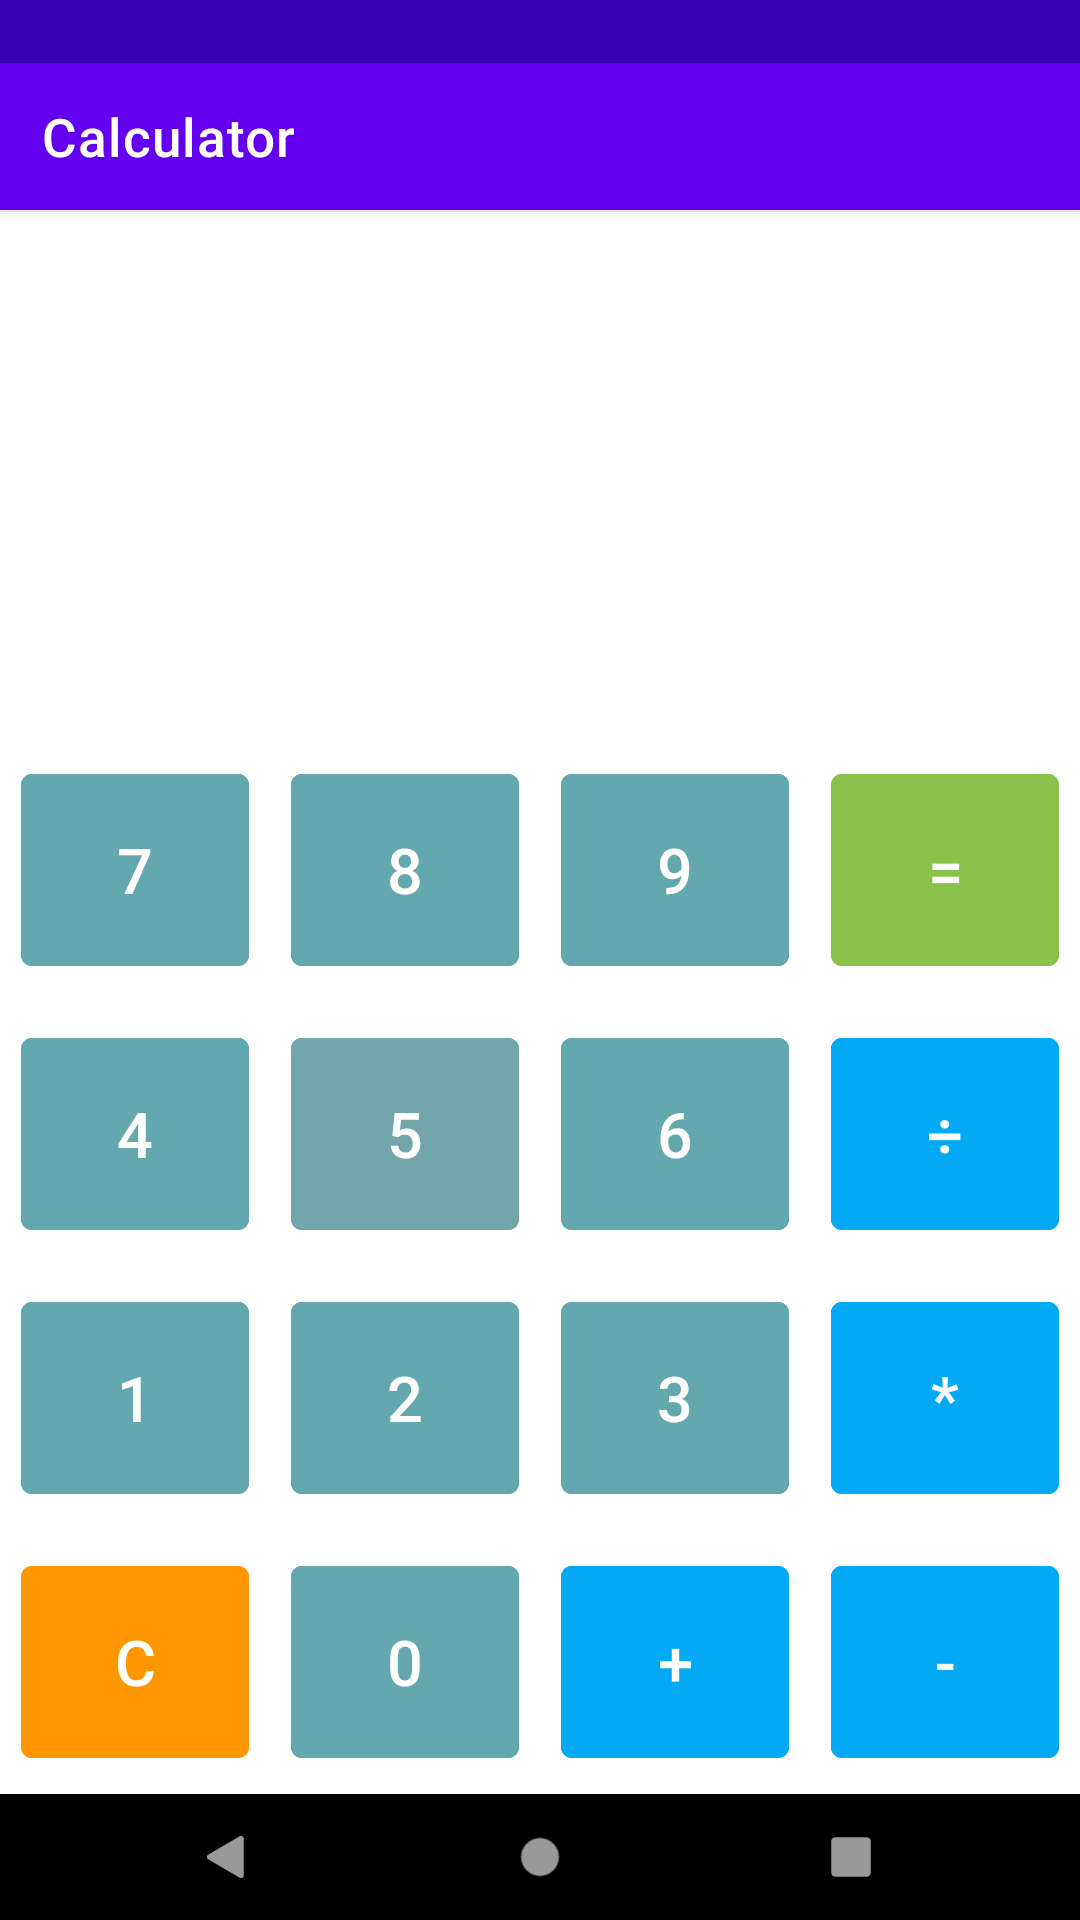
\includegraphics[width=5cm, height=9cm]{../tex/img/practicals/02-calculator-1.png}  \\

\textbf{Note:} each number \& operator in the example above is a \textbf{Button} widget.

\subsection*{Task Two (0.5\%):} 
The application's \textbf{action bar} displays the activity's \textbf{title} on the top left-hand side \& an overflow menu on the top right-hand side. Create a new resource directory called \textbf{menu}. To do this, right-click on \textbf{res $>$ Android Resource Directory}. In the \textbf{New Resource Directory} window, change the \textbf{Directory name} \& \textbf{Resource type} to \textbf{menu}. In the \textbf{menu} directory, create a new \textbf{XML} file called \textbf{menu}. Use the following resource to define a menu - \href{https://developer.android.com/guide/topics/ui/menus}{https://developer.android.com/guide/topics/ui/menus} \\

To specify the options menu for an activity, i.e., \textbf{MainActivity.kt}, override the \textbf{onCreateOptionsMenu()} method. In this method, inflate your \textbf{menu} resource defined in \textbf{menu.xml} into the \textbf{Menu} provided in the callback. For example:

\begin{verbatim}
    override fun onCreateOptionsMenu(menu: Menu): Boolean {
        val inflater = menuInflater
        inflater.inflate(R.menu.menu, menu)
        return true
    }
\end{verbatim}

Run your application on either an \textbf{Android Emulator} or \textbf{connect device}. You should see a vertical ellipsis on the top right-hand side. This is your inflated \textbf{menu} resource mentioned above. \\

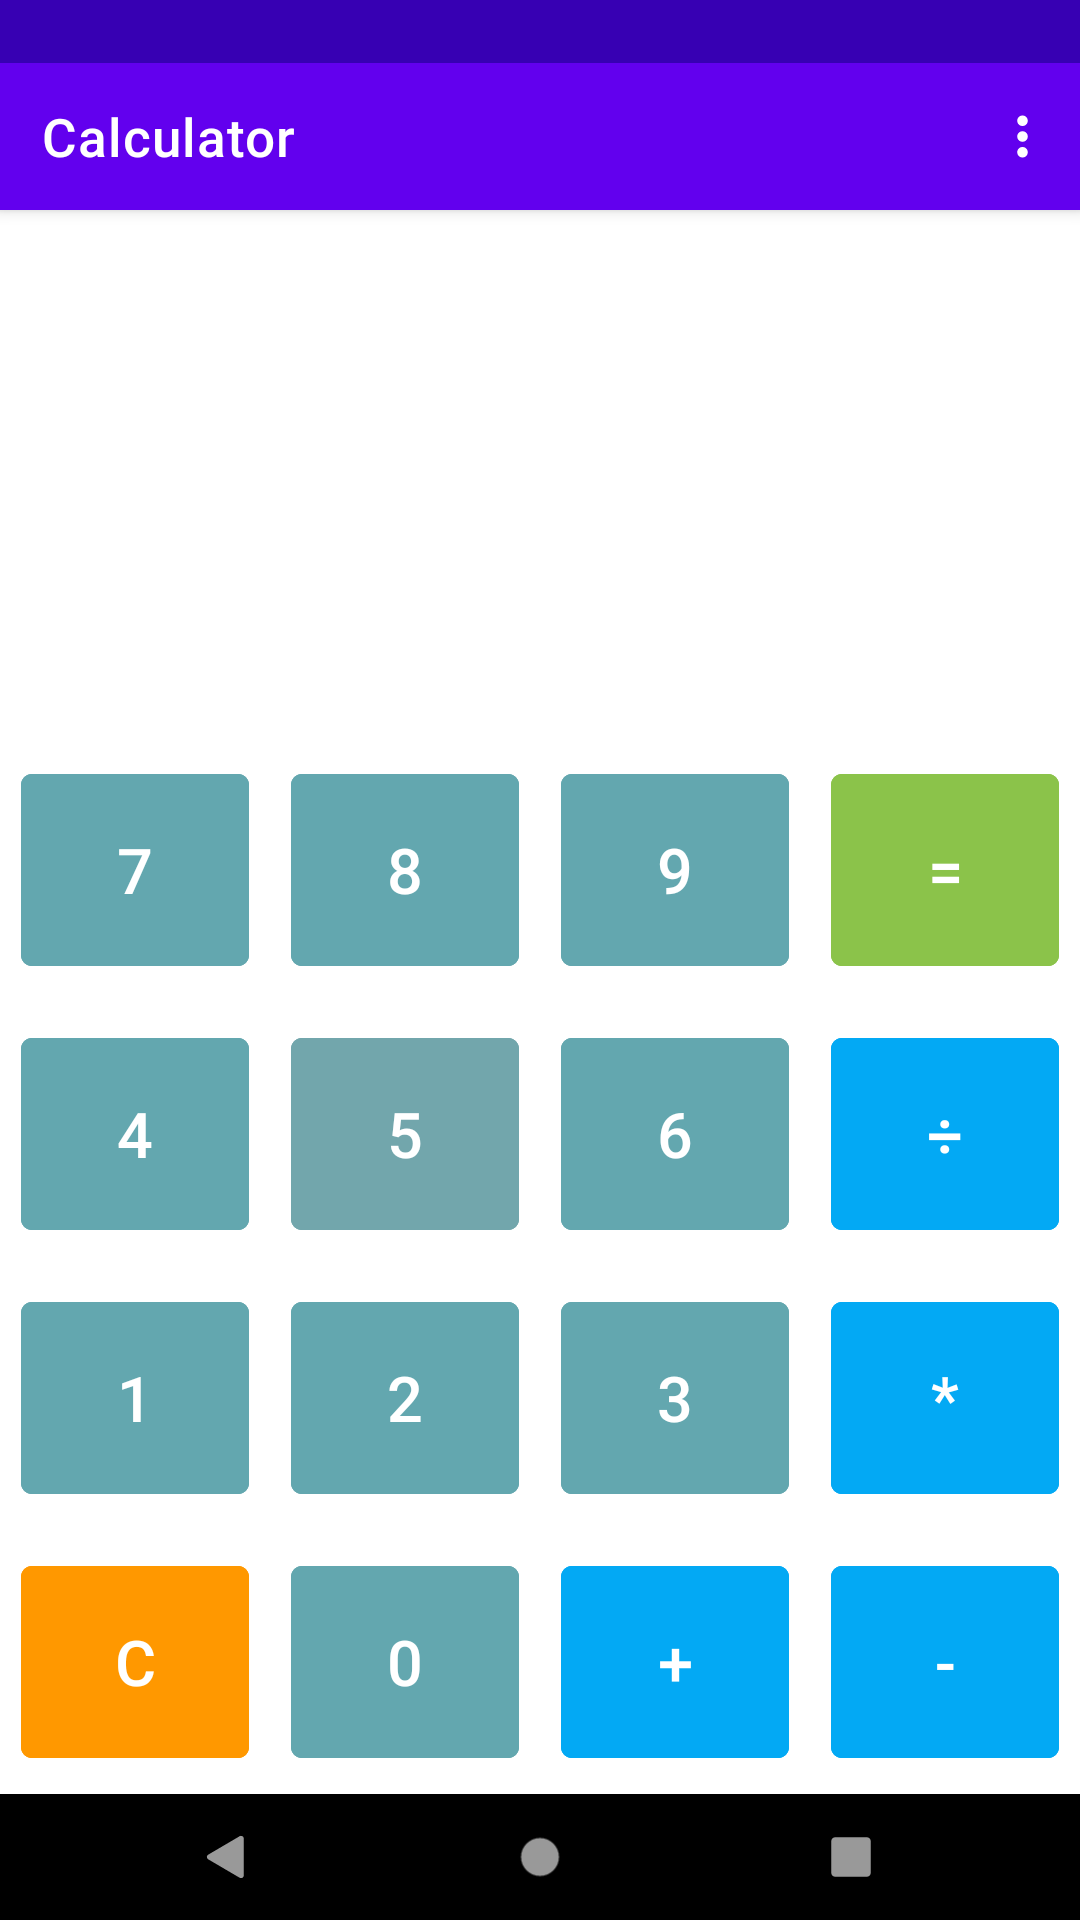
\includegraphics[width=5cm, height=9cm]{../tex/img/practicals/02-calculator-2.png}

\subsection*{Task Three (2\%):} 
In \textbf{MainActivity.kt}, write code that allows your application to function as a calculator. If you wish, you can use third-party libraries. However, it is encouraged that you write the functionality from scratch. \\

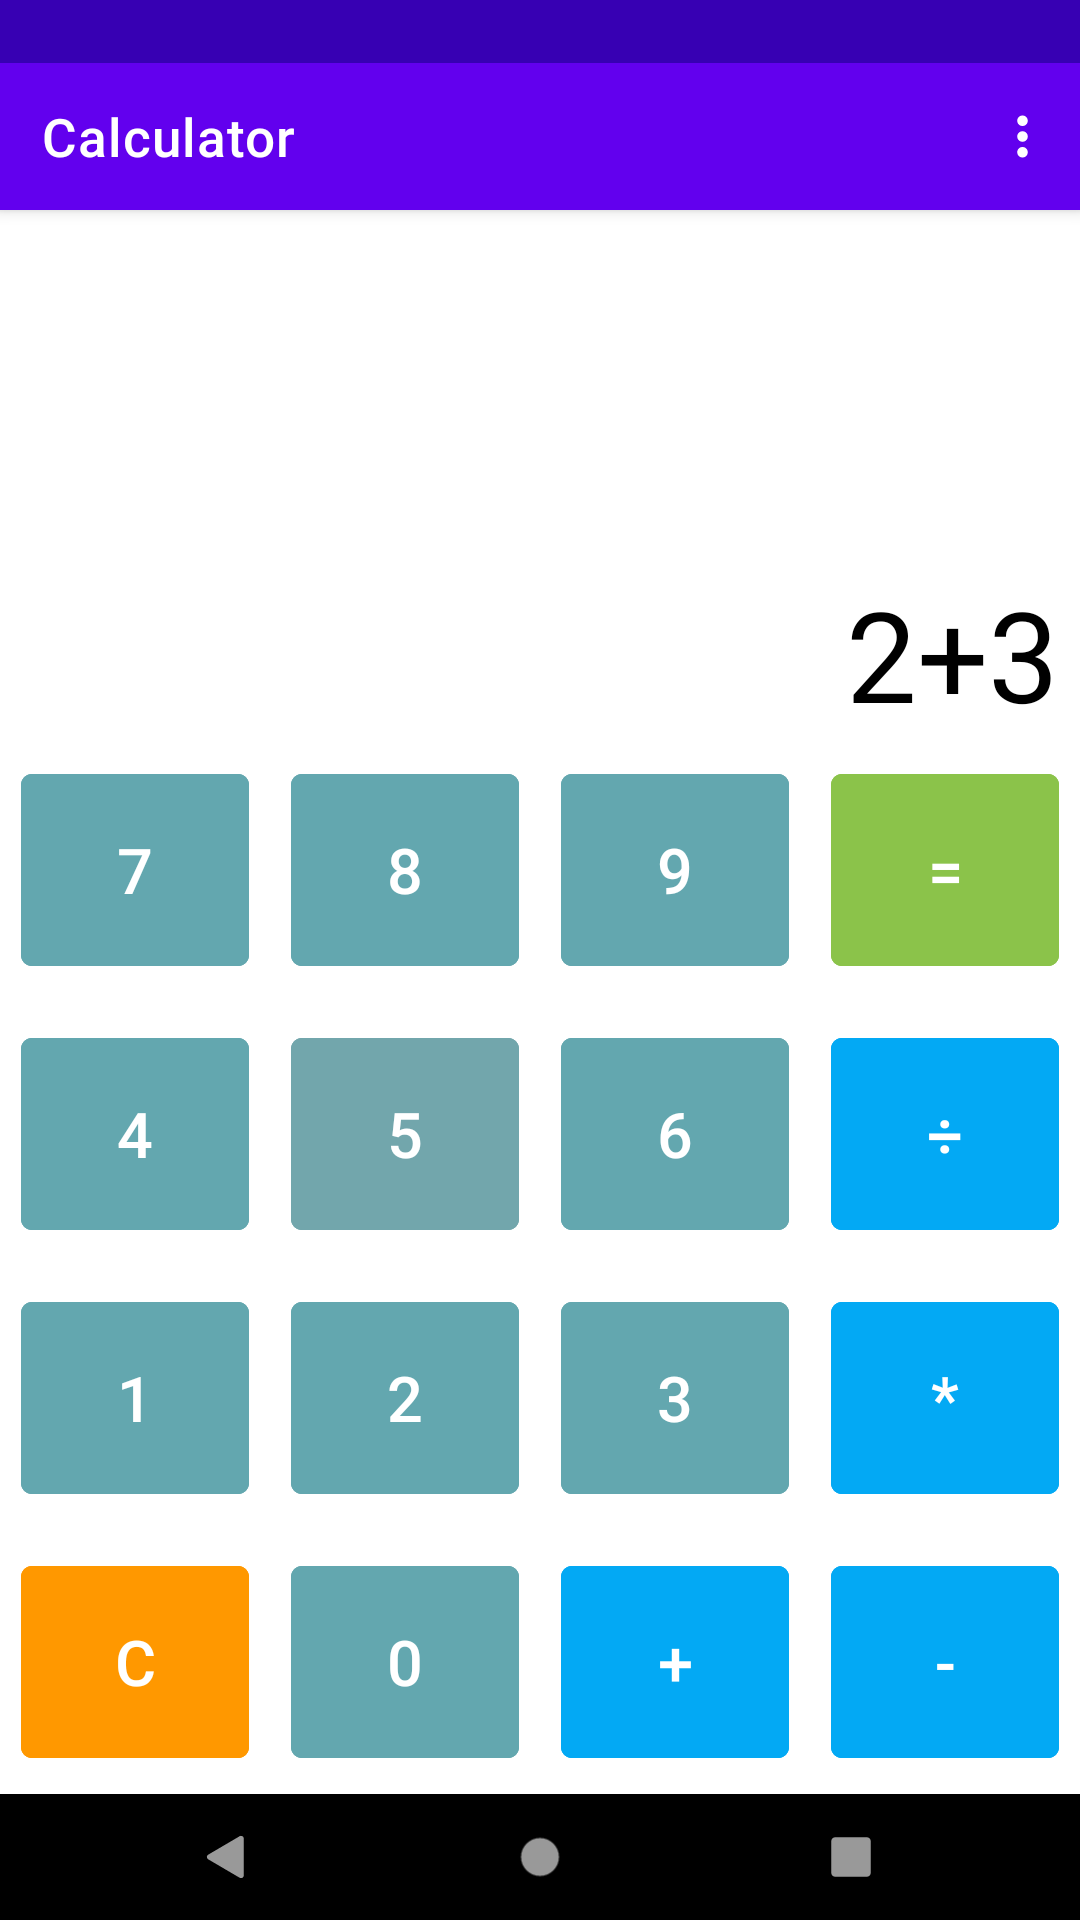
\includegraphics[width=5cm, height=9cm]{../tex/img/practicals/02-calculator-3.png}
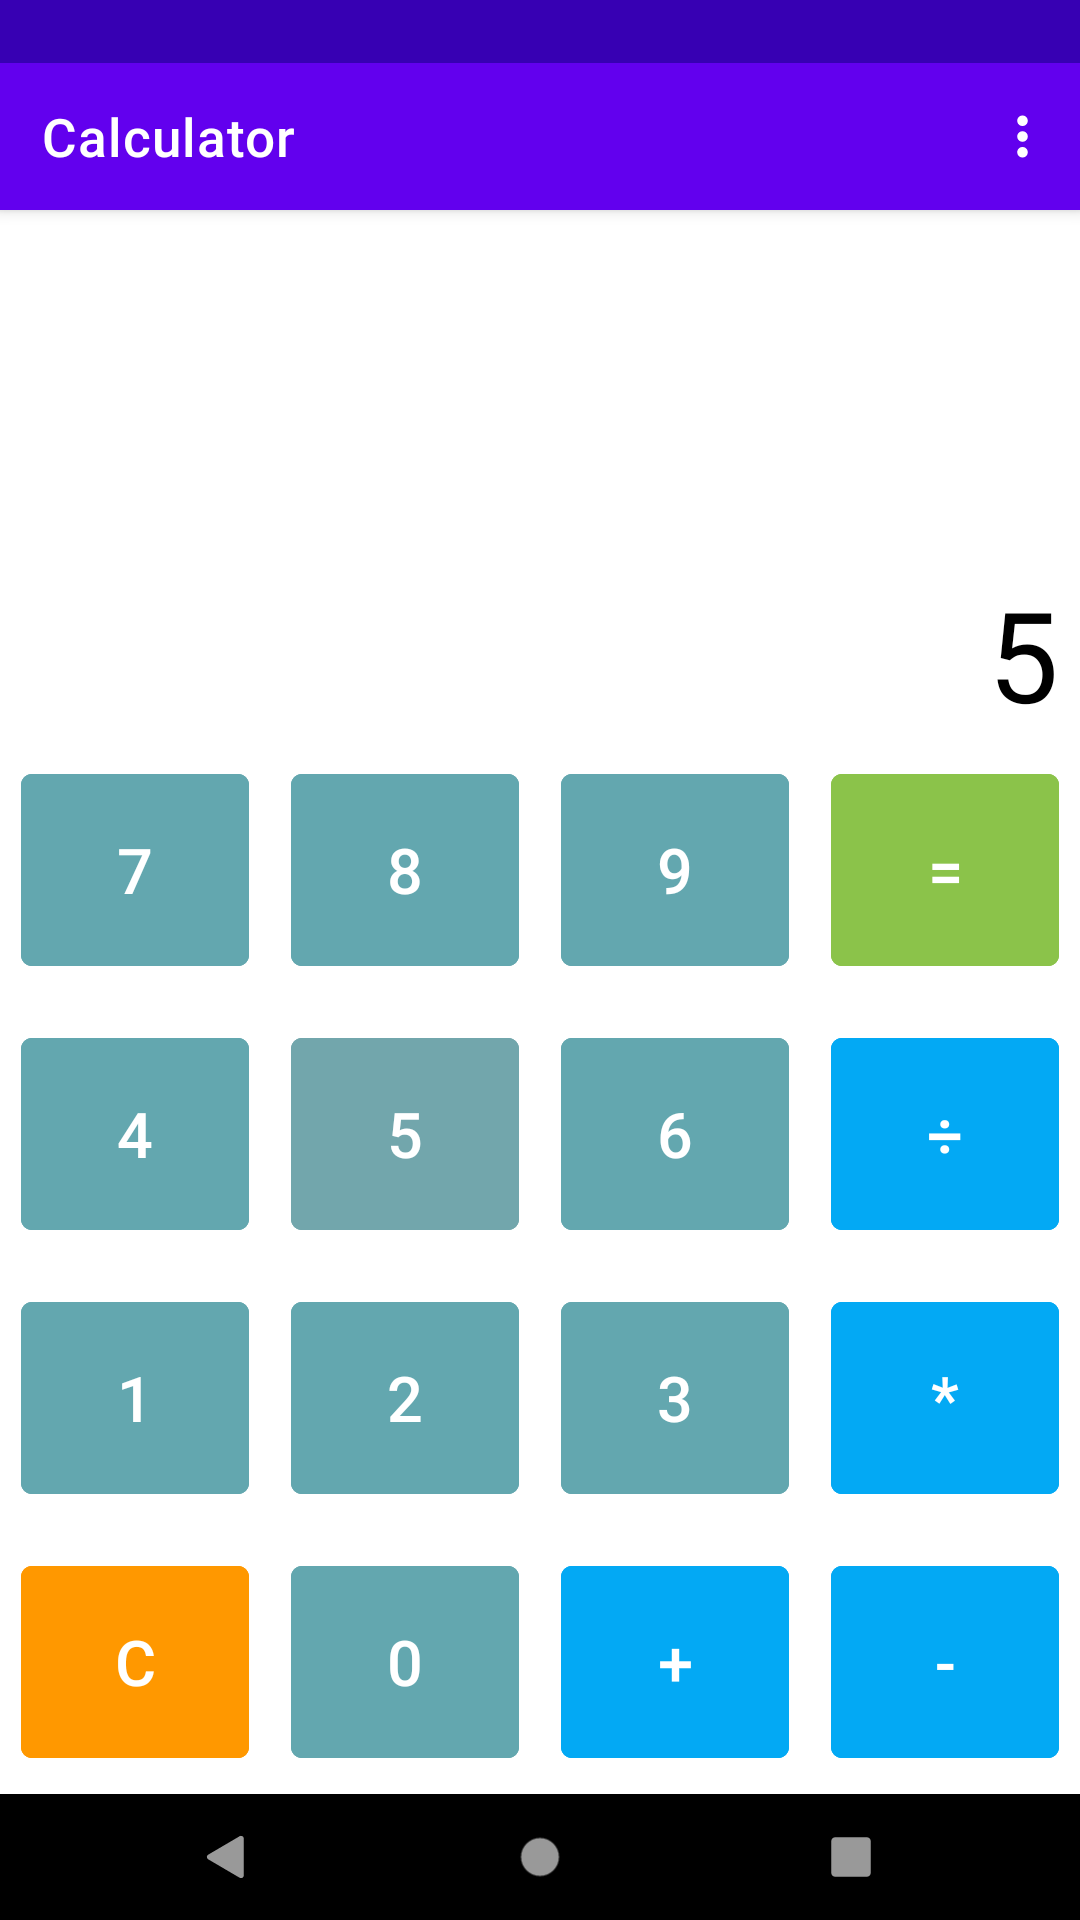
\includegraphics[width=5cm, height=9cm]{../tex/img/practicals/02-calculator-4.png} \\

Where possible, write code that checks for potential calculation errors. For example, dividing by zero should return \textbf{NaN} or \textbf{undefined}. \\

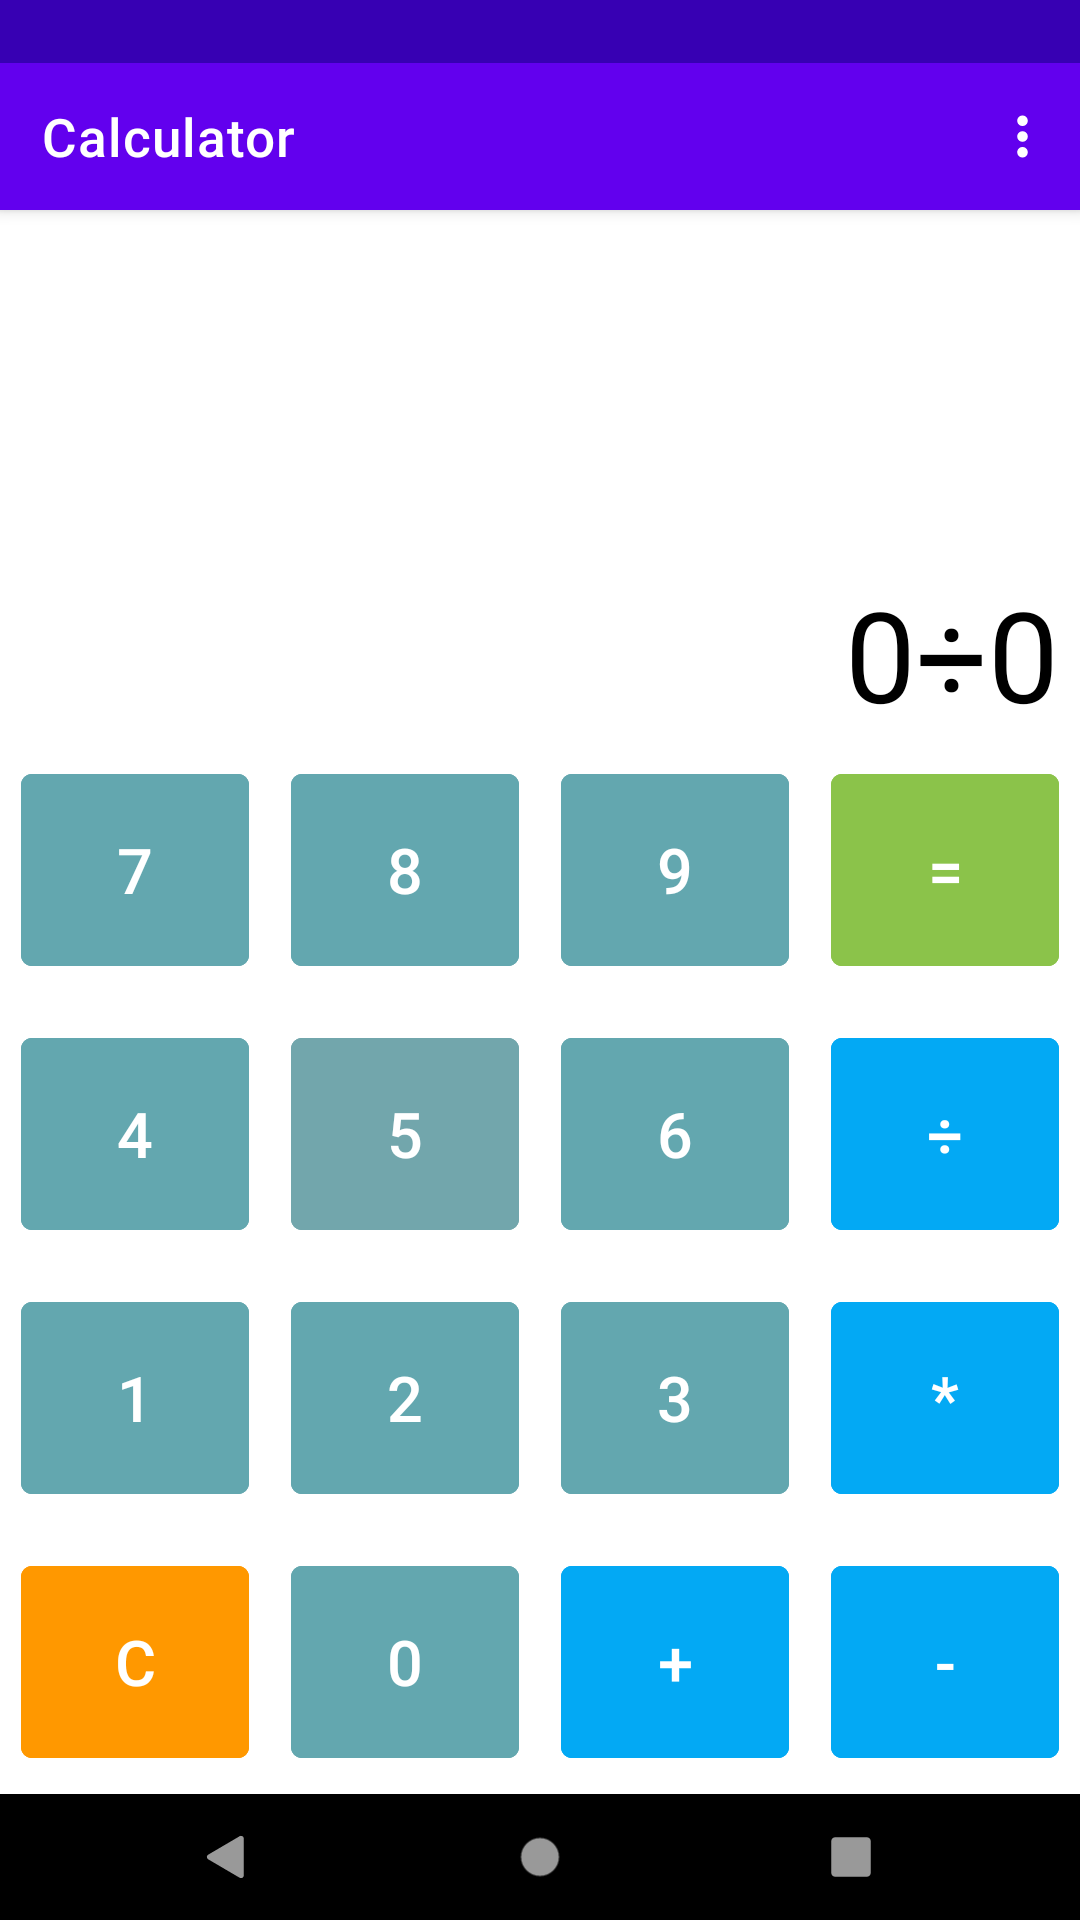
\includegraphics[width=5cm, height=9cm]{../tex/img/practicals/02-calculator-5.png}
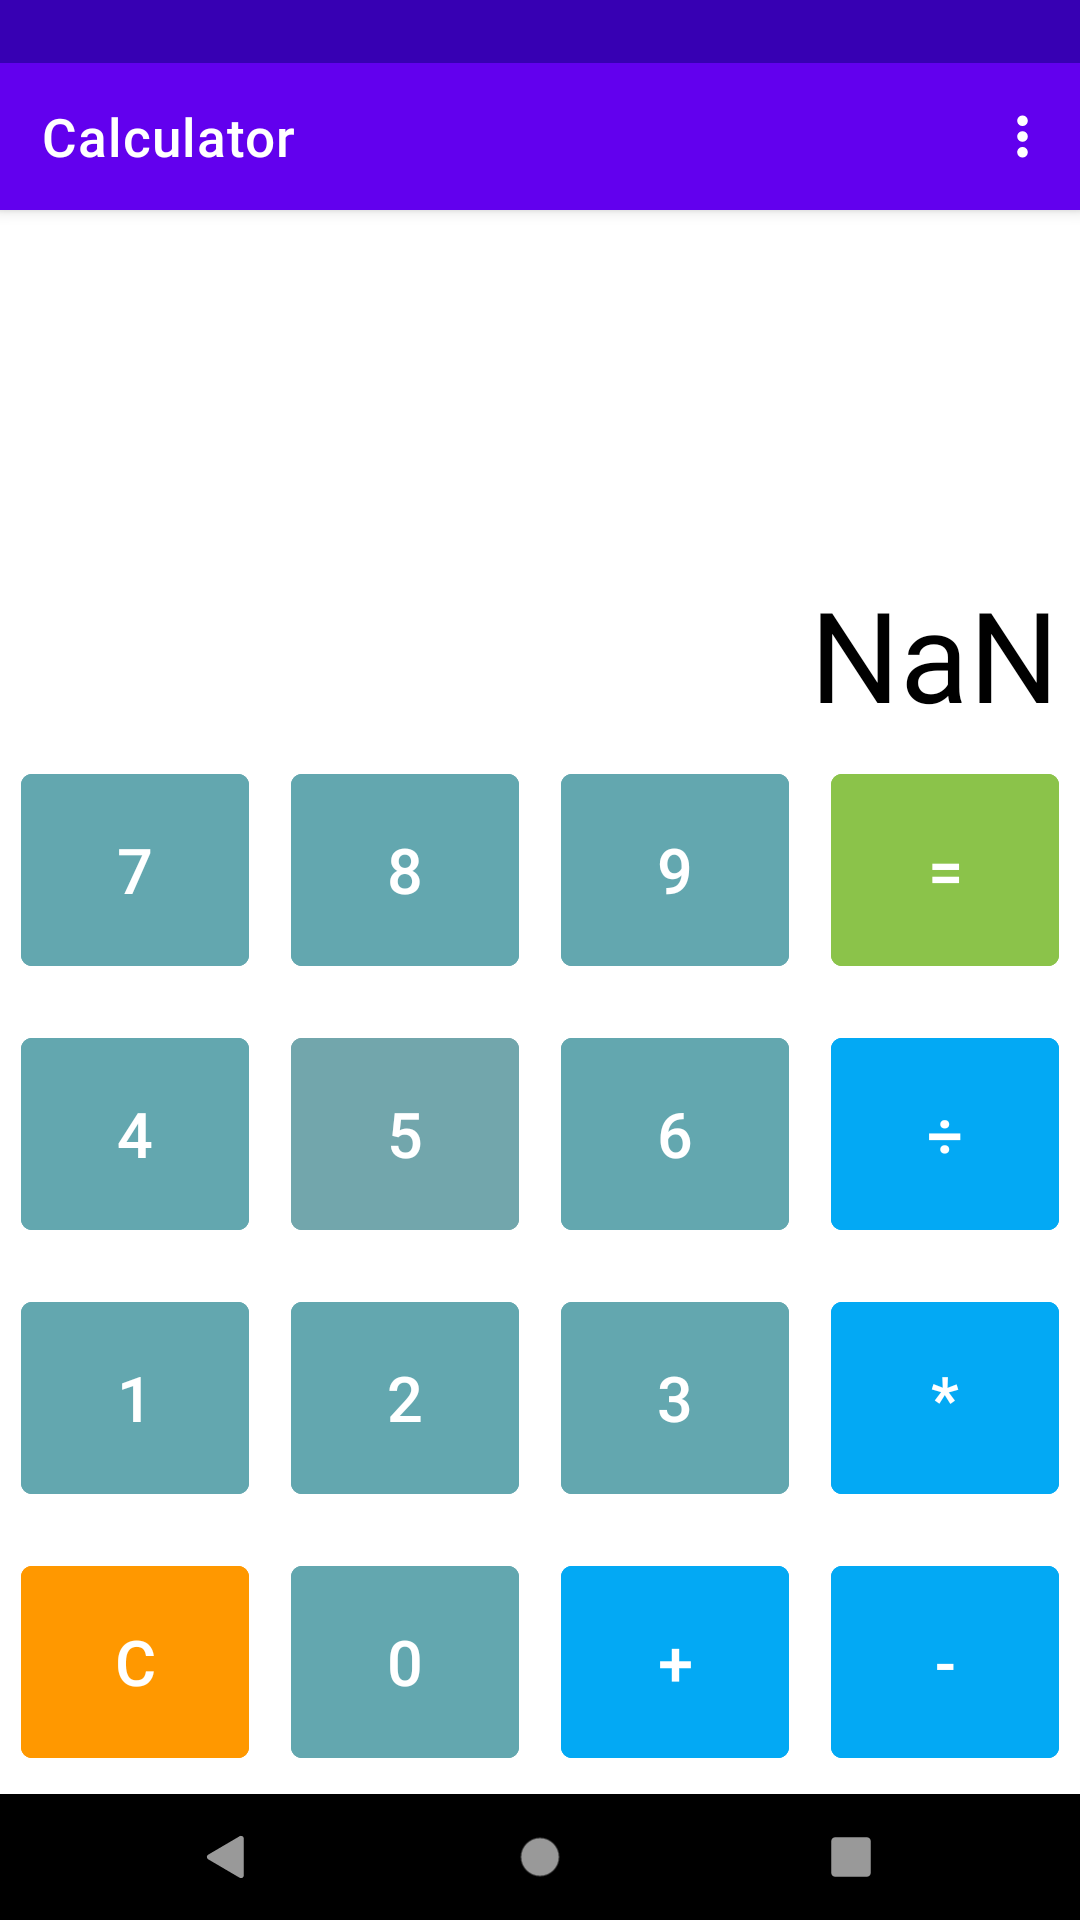
\includegraphics[width=5cm, height=9cm]{../tex/img/practicals/02-calculator-6.png}

\subsection*{Task Four (1\%):} 
One method to UI testing is to have a person perform a set of tasks on a target application \& verify that it is behaving correctly. However, this manual method is time-consuming \& error-prone. A more efficient method is to write UI tests that perform such tasks in an automated way. \\

Create a new test file called \textbf{CalculatorTest}. To do this, right-click on \textbf{op.mobile.app.dev.calculator (androidTest) $>$ Kotlin Class/File}. In \textbf{CalculatorTest.kt}, write UI tests for the following cases:

\begin{itemize}
	\item Calculate two numbers. \textbf{Note:} any operator will be sufficient.
	\item Output of the calculation. For example, if you add 2 \& 4, you should expect the output to be 6.
	\item Calculate two numbers using the divide operator so that the output is \textbf{NaN} or \textbf{undefined}.
\end{itemize}

To run your test file, right-click \textbf{CalculatorTest.kt $>$ 'Run CalculatorTest'}.

\end{document}